% !TEX root = gmin332.tex

\section{TD 6}
\subsection{Enoncé}

\subsubsection{Diagramme de classes}
\begin{figure}[H]
  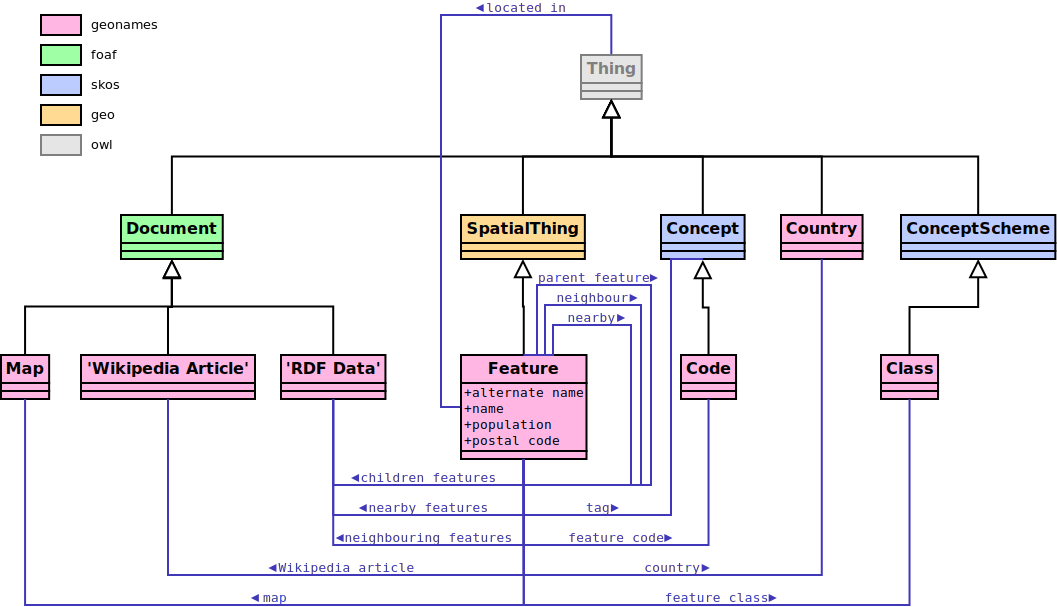
\includegraphics[width=\textwidth]{../diag_class}
  \caption{Diagramme de classes de l'ontologie Géonames (Lite).}
\end{figure}

\subsection{Questions}
\subsubsection{Question 1}
\begin{verbatim}
PREFIX rdfs:<http://www.w3.org/2000/01/rdf-schema#>
PREFIX owl:<http://www.w3.org/2002/07/owl#>
PREFIX rdf:<http://www.w3.org/1999/02/22-rdf-syntax-ns#>
PREFIX core:<http://www.w3.org/2004/02/skos/core#>
PREFIX ontology:<http://www.geonames.org/ontology#>

SELECT ?subject ?Class ?prefLabel ?definition
where {
  ?subject rdf:type ontology:Code .
  OPTIONAL {
    ?subject core:inScheme ?Class
  } .
  OPTIONAL {
    ?subject core:prefLabel ?prefLabel .
    FILTER (lang(?prefLabel) = "" || lang(?prefLabel) = "en")
  }
  OPTIONAL {
    ?subject core:definition ?definition .
    FILTER (lang(?definition) = "" || lang(?definition) = "en")
  }
}
\end{verbatim}
Type de jointure : S-S Patron de graphe : Étoile
%%
\subsubsection{Question 2}
\begin{verbatim}
PREFIX rdfs:<http://www.w3.org/2000/01/rdf-schema#>
PREFIX owl:<http://www.w3.org/2002/07/owl#>
PREFIX rdf:<http://www.w3.org/1999/02/22-rdf-syntax-ns#>
PREFIX core:<http://www.w3.org/2004/02/skos/core#>
PREFIX ontology:<http://www.geonames.org/ontology#>

SELECT ?subject ?definition
where {
  ?subject core:inScheme ontology:V .
  OPTIONAL {
    ?subject core:definition ?definition .
    FILTER (lang(?definition) = "" || lang(?definition) = "en")
  }
}
\end{verbatim}
Type de jointure : S-S Patron de graphe : Étoile
%%
\subsubsection{Question 3}
\begin{verbatim}
PREFIX rdfs:<http://www.w3.org/2000/01/rdf-schema#>
PREFIX owl:<http://www.w3.org/2002/07/owl#>
PREFIX rdf:<http://www.w3.org/1999/02/22-rdf-syntax-ns#>
PREFIX core:<http://www.w3.org/2004/02/skos/core#>
PREFIX ontology:<http://www.geonames.org/ontology#>

SELECT ?subject (COUNT(DISTINCT ?code) AS ?nb)
where {
  ?subject rdf:type ontology:Class .
  ?code core:inScheme ?subject 
} GROUP BY ?subject
\end{verbatim}
\subsubsection{Question 4}
\begin{verbatim}
PREFIX rdfs:<http://www.w3.org/2000/01/rdf-schema#>
PREFIX owl:<http://www.w3.org/2002/07/owl#>
PREFIX rdf:<http://www.w3.org/1999/02/22-rdf-syntax-ns#>
PREFIX core:<http://www.w3.org/2004/02/skos/core#>
PREFIX ontology:<http://www.geonames.org/ontology#>

SELECT ?code ?def
where {
  ?code rdf:type ontology:Code .
  ?code core:definition ?def .
  FILTER CONTAINS(?def, "ice")
}
\end{verbatim}
\subsubsection{Question 5}
\begin{verbatim}
PREFIX rdfs:<http://www.w3.org/2000/01/rdf-schema#>
PREFIX owl:<http://www.w3.org/2002/07/owl#>
PREFIX rdf:<http://www.w3.org/1999/02/22-rdf-syntax-ns#>
PREFIX core:<http://www.w3.org/2004/02/skos/core#>
PREFIX ontology:<http://www.geonames.org/ontology#>

SELECT ?name ?url
where {
  <http://sws.geonames.org/2985244/> ontology:parentFeature ?parent .
  ?neighbours ontology:parentFeature ?parent .
  ?neighbours ontology:name ?name .
  ?neighbours rdfs:isDefinedBy ?url
}
\end{verbatim}
Retourne les voisins d'une feature (ici http://sws.geonames.org/2985244/) en sélectionnant le père et en récupérant les fils. Sélection du nom de chaque feature et son url (isDefinedBy).
%%
\subsubsection{Question 6}
\begin{verbatim}
PREFIX rdfs:<http://www.w3.org/2000/01/rdf-schema#>
PREFIX owl:<http://www.w3.org/2002/07/owl#>
PREFIX rdf:<http://www.w3.org/1999/02/22-rdf-syntax-ns#>
PREFIX core:<http://www.w3.org/2004/02/skos/core#>
PREFIX ontology:<http://www.geonames.org/ontology#>

SELECT ?s
where {
  ?p rdf:type owl:ObjectProperty .
  ?p rdfs:range ontology:Feature .
  ?s ?p ?o
}
\end{verbatim}
Sélection de toutes les entités qui ont au moins une relation avec une feature (relation ayant comme range Feature).

\subsection{2. Questions sur le modèle}

    Une feature au sens géonames peut admettre plusieurs codes, étant donné qu'aucune contrainte de cardinalité n'est définie dans l'ontologie.
    Geonames utilise qu'une faible partie de skos pour définir ses concepts. On y retrouve l'utilisation des ckasses de scheme et de concept (et donc la relation inScheme), ainsi que les comments et prefLabel. Mais aucune hiérarchie ni relations entre concepts ne sont définies (broader / narrower / related / etc...).
    La classe la moins décrite dans l'ontologie géonames est la classe Country. En effet elle n'hérite d'aucune classe et n'est donc définie que par un commentaire et un label.
